\section{Proses Pembuatan Aplikasi}
Metode proses pembuatan software iterative adalah pendekatan pengembangan perangkat lunak yang dilakukan secara bertahap melalui siklus pengulangan (iterasi). 
Setiap iterasi mencakup seluruh tahapan pengembangan perangkat lunak, mulai dari perencanaan, analisis, desain, pengembangan, hingga pengujian dan evaluasi. 
Berikut adalah penjelasan lebih detail mengenai metode ini:

\begin{figure}[H]
    \centering
    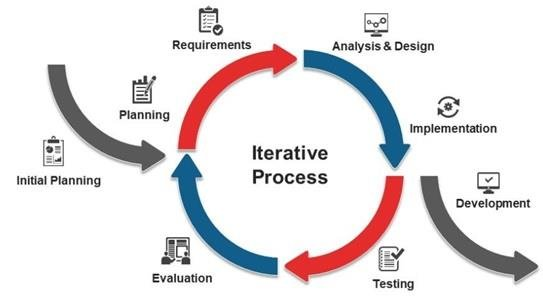
\includegraphics[width=0.8\textwidth]{assets/iterative.jpg}
    \caption{Proses Iterasi}
\end{figure}

\subsection{Iterasi Pertama}
Periode Iterasi : (2 July 2024 - 10 July 2024)

Beranjak dari problem yang ada dalam latar belakang. Kami menyusun MVP yang ada dimana pada minimalnya
aplikasi harus bisa menampilkan konten, menambahkan konten dengan admin panel. Memutar lagu. Menampilkan sejarah yang ada
dan aplikasi harus open source. Dimana siapa saja dapat berkontribusi ke aplikasi ini. Kemudian karena itu kami menetapkan 
list fitur iterasi pertama sebagai berikut.

\begin{itemize}
    \item Onboarding
    \item Home Page
    \item List of Tembang
    \item Karaoke Player
    \item Information Detail
\end{itemize}

\subsection{Iterasi Kedua}
Periode Iterasi : (Start 1 Agustus 2024)

Dengan melihat hasil kritik dan saran yang diterima dari presentasi aplikasi kami pada acara
Kreativnesia Badung 2024 mulai dari kerisauan tentang bagaimana penyampaian aplikasi ini kepada masyarakat.
Kerisauan pada jumlah konten yang ada, keamanan serta kritik dan saran lain yang didapatkan dari tim internal.
Mulai dari dark mode yang untuk memberi tambahan kenyamanan pada pembaca. Dan juga jawaban dari masalah
selling point aplikasi yaitu gamification system. Berikut kami list fitur yang akan dibuat adalah sebagai
berikut.

\begin{itemize}
    \item Gamification System
    \item Dark Mode
    \item Favourite
    \item All Song + Search + Filter
    \item Profile
\end{itemize}

